\documentclass{article}
\usepackage{subcaption}


% Language setting
% Replace `enapplicationglish' with e.g. `spanish' to change the document language
\usepackage[english]{babel}

% Set page size and margins
% Replace `letterpaper' with `a4paper' for UK/EU standard size
\usepackage[letterpaper,top=2cm,bottom=2cm,left=3cm,right=3cm,marginparwidth=1.75cm]{geometry}

% Useful packages
\usepackage{amsmath}
\usepackage{graphicx}
\usepackage[colorlinks=true, allcolors=blue]{hyperref}

\title{MoSIS Assignment 2: CBD}
\author{Stein Vandenbroeke s0205627 & Niels Van den Broeck s0203844}

\begin{document}
\maketitle


\section{Integration Methods}

\subsection{Implementation of Integration methods}
The first part of the assignment is about implementing integrators. Before we jumped into the creation of the different integrator methods, we made a simple test in DrawIo with a clock attached to it to check whether the DrawIoConvert and CBD work correctly. \\

After getting everything setup correctly, we started with the Backwards Euler Method. The integrator works by adding a block of a certain area for each timestamp. At time $t_{i}$, it takes the value of $f(t_{i-1})$ and multiplies it with $\delta t$ to get the desired area of the rectangle. To accomplish this in CBD, we drew the block diagram in DrawIo which is shown in Figure \ref{fig:backwards_euler}. There are 2 delay blocks present. One is mandatory to store the integral (areas) of all previous timestamps. You can see that the result of the current timestamp goes to the output, as well as to the delay block for the next timestamp. This value is then used to add to the new area. The other Delay is needed to get the value of $f(t_{i-1})$. Because we are in timestamp $t_{i}$, we don't have direct access to $t_{i-1}$ and thus a delay is used. Since we use the value of $t_{i-1}$, at time $t_{i}$, we need to add an edge case for the first iteration. at $t_{0}$, we do not want to do anything, so we pass it through the delay block which takes the initial condition value which is set by the user (mostly zero). From the next timestamp on, it will take the previous calculated values.\\

\begin{figure}
    \centering
    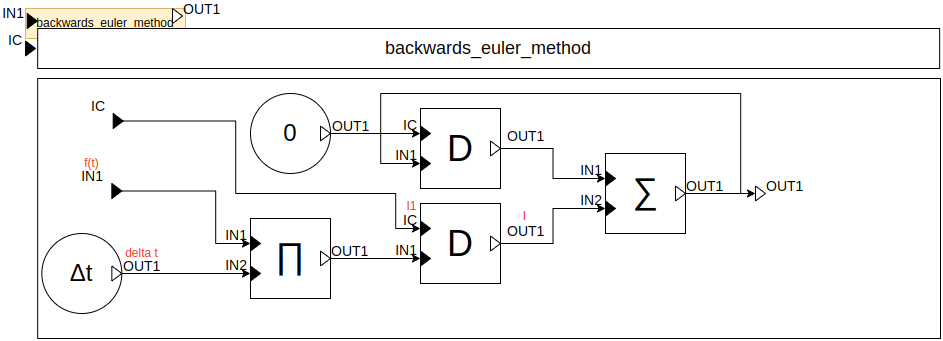
\includegraphics[width=0.75\linewidth]{Images/Backwards_Euler_Method.drawio.png}
    \caption{Backwards Euler Method}
    \label{fig:backwards_euler}
\end{figure}

The second method, named the Forwards Euler Method, is not much different to the Backwards Euler Method. Instead of taking the value of $f(t_{i-1})$ to calculate the area of the block, we use $f(t_{i})$. This results in no longer needing the delay block to hold $f(t_{i-1})$. As you can see in Figure \ref{fig:forwards_euler}, there is only 1 delay block present. in Backwards Euler Method, the edge case for $t_{0}$ was handled by the delay block. For the Forward Euler Method, we have to handle this a bit differently. Again, we don't want to calculate anything at $t_{0}$, so we simply take the negative of the resulted area and put them in the initial condition, this will run only at time $t_{0}$ and thus it will cancel out at the addition.\\

\begin{figure}
    \centering
    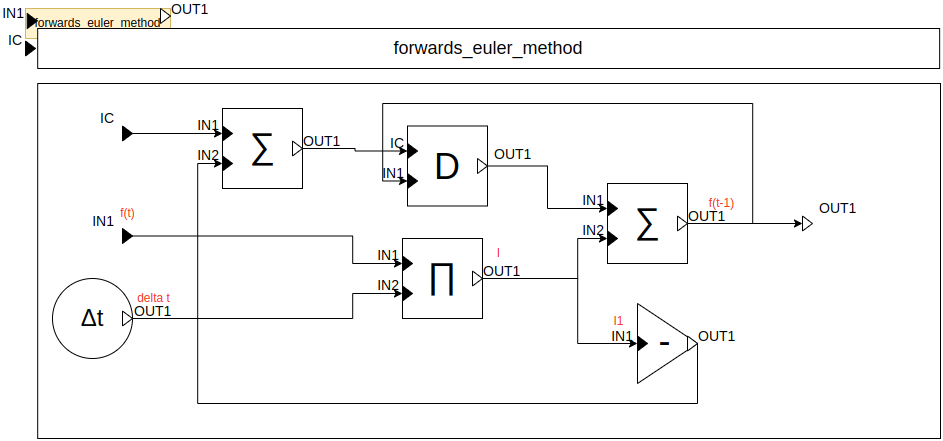
\includegraphics[width=0.75\linewidth]{Images/Forward_Euler_Method.drawio.png}
    \caption{Forwards Euler Method}
    \label{fig:forwards_euler}
\end{figure}

The Trapezoid Rule works a bit differently. At timestamp $t_{i}$, it adds the values of $f(t_{i})$ and $f(t_{i-1})$ and divides it by 2, followed by a multiplication of $\delta t$. The usage of $t_{i}$ as well as $t_{i-1}$ and the multiple additions and multiplications, make the block diagram seem a bit complicated, but overall, it has the same idea. For dealing with the first timestamp $t_{0}$, we used the same method as for the Forward Euler Method where we subtract the area with itself for the initial condition only. The block diagram is shown in Figure \ref{fig:trapezoid_rule}.\\

\begin{figure}
    \centering
    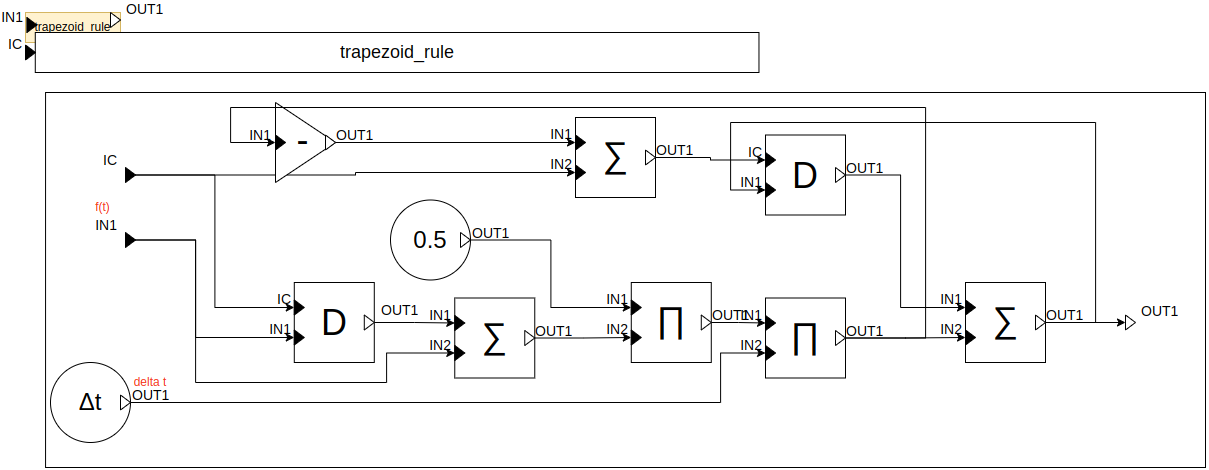
\includegraphics[width=0.75\linewidth]{Images/Trapezoid_Rule.drawio.png}
    \caption{Trapezoid Rule}
    \label{fig:trapezoid_rule}
\end{figure}

\subsection{Implementation of test functions}

To actually test whether our integration methods work as desired, we created a function to pass in our integrator block. Before doing this, we made a simple example by passing the time as a function, which simulates the function x. We checked the output of our Backwards Euler method with the already implemented integrator method and we got the same results. Next, we implemented the function $g(t) = \frac{t + 2}{(t + 3)^2}$ which is shown in Figure \ref{fig:g_function}. In the assignment, it is stated that the integral of the function $g(t)$ between 0 and 100 is approximately the same as the integral of another function $g_2(t)$ between 3 and 103. We implemented the $g_2(t)$ and confirmed that this is the case. Since this was for testing purposes only, we added 3 to the time in our block diagram so that we do not have to handle the different starting and ending point. The block diagram of $g_2(t)$ can be found in Figure \ref{fig:g_2_function}.\\

\begin{figure}
    \centering
    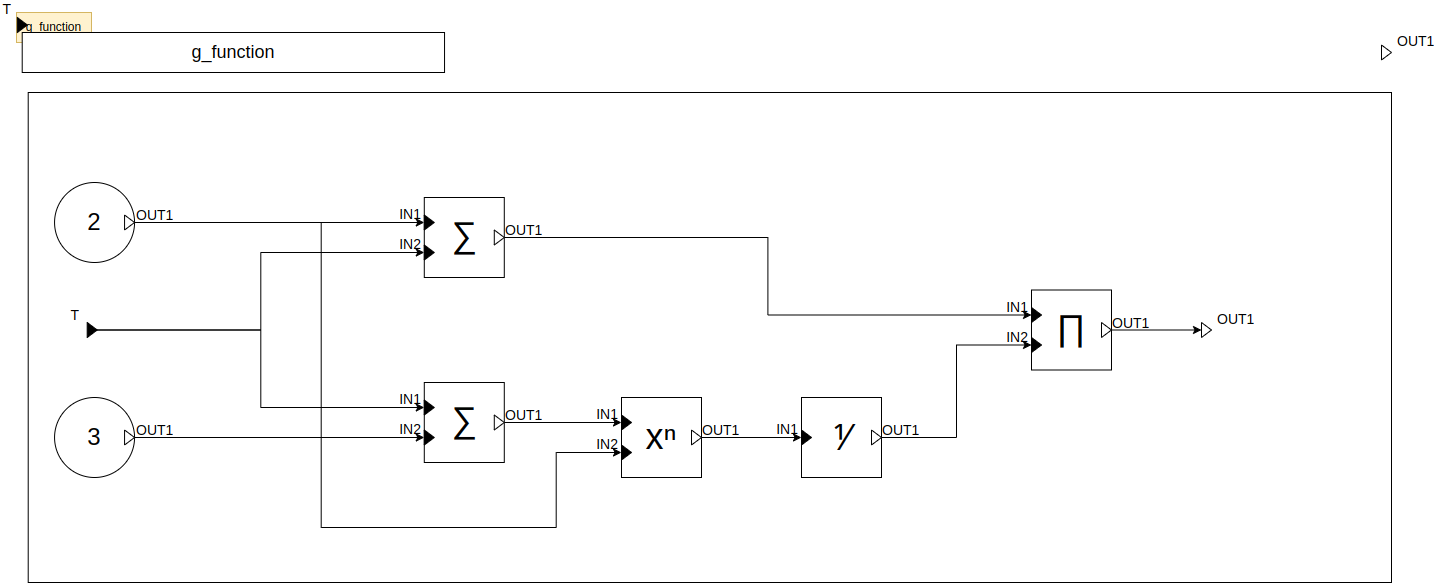
\includegraphics[width=0.75\linewidth]{Images/g_Function.drawio.png}
    \caption{Function $g(t)$}
    \label{fig:g_function}
\end{figure}

\begin{figure}
    \centering
    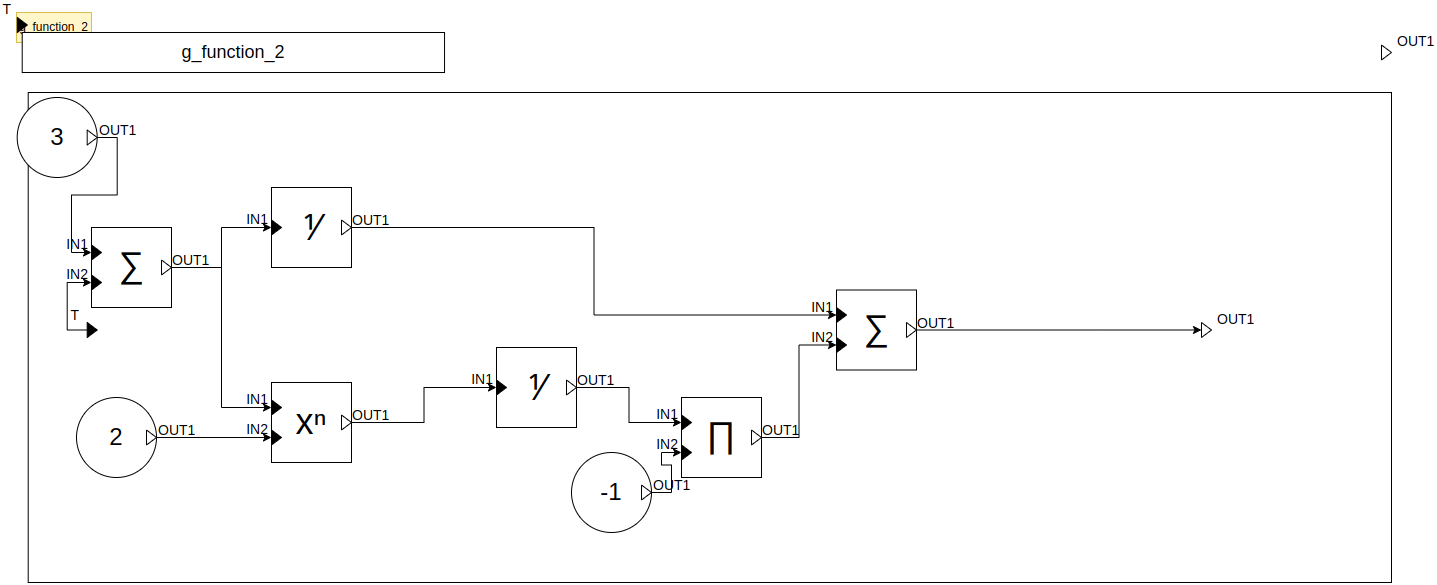
\includegraphics[width=0.75\linewidth]{Images/g_Function_2.drawio.png}
    \caption{Function $g_2(t)$}
    \label{fig:g_2_function}
\end{figure}

\subsection{Results}

Now that we have our 3 integrator methods and a function to calculate the integration for a specified interval, we can compare the outcomes for different delta times:

\begin{center}
    \begin{tabular}{ c | c c c | c}
         $\delta t$ & Backward & Forward & Trapezoid & Analytical solution \\ 
         \hline
     0.1 & 3.222190908 & 3.200931059 & 3.211560984 & \\ 
     0.01 & 3.213459296 & 3.211333228 & 3.212396262 & \\
     0.001 & 3.212588796 & 3.212376188 & 3.212482492 & \\
     \hline
     &&&&3.212492104
    \end{tabular}
\end{center}

These results are not unexpected. As visible in Figure \ref{fig:g_function_plot}, the function is descending in the interval [0,100]. If we use the Backwards Euler Method, it takes the first value of the iteration, which is higher than the second value due to the descending function, and thus overshoots a little bit. This concludes in a higher value for the integration than the actual analytical value. The Forwards Euler Method works the other way around. It takes the second value which is smaller than the first and thus it undershoots and returns a smaller value than the actual analytical value. Lastly, the Trapezoid Rule tries to mimic the curve of the function. This could be inaccurate in cases where the first and second timestamp values are approximately the same, but where there is a huge fluctuation in between. Fortunately, this is not the case in the interval of our function, so the Trapezoid Rule is fairly accurate.

\begin{figure}
    \centering
    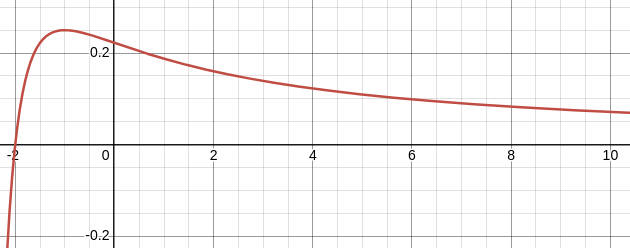
\includegraphics[width=0.75\linewidth]{Images/g_function_plot.png}
    \caption{Function $g(t)$}
    \label{fig:g_function_plot}
\end{figure}

\section{CO-simulation}
\subsection{PID controller}
Creating the PID controller (see Figure \ref{fig:PID-controller}) was relatively easy because of the experience from the previous assignment. The Kp, Ki and Kd variables were set to 26,1,10 (the same values as Assignment 1 except for the Ki value that is now 1 instead of the original 0). We created the PID in DrawIo and then converted it into CBD python code using the DrawioConvert. Now that we have the python CBD, we want to create an FMU of the PID controller (using CBD2FMU). This will convert the python CBD to C code which is faster and more efficient and is compiled so competitors can easily use the PID controller (with the standard FMI) in their own system without seeing the source code. 
The CBD2FMU gave us an FMU which can be extracted. When we review the content inside, we find the description.xml, sources/model.c files. The description.xml file contains the C code source files, some experiment data and all flattened ModelVariables. In the model.c, there are several important functions:
\begin{itemize}
  \item initialEquations: Sets all flattened equations for the first iteration (based on how the blocks are connected).
  \item calculateEquations: Sets all flattened variables (equations) for all other iterations (based on how the blocks are connected).
  \item doStep: Allows to loop over time.
\end{itemize}
\begin{figure}
    \centering
    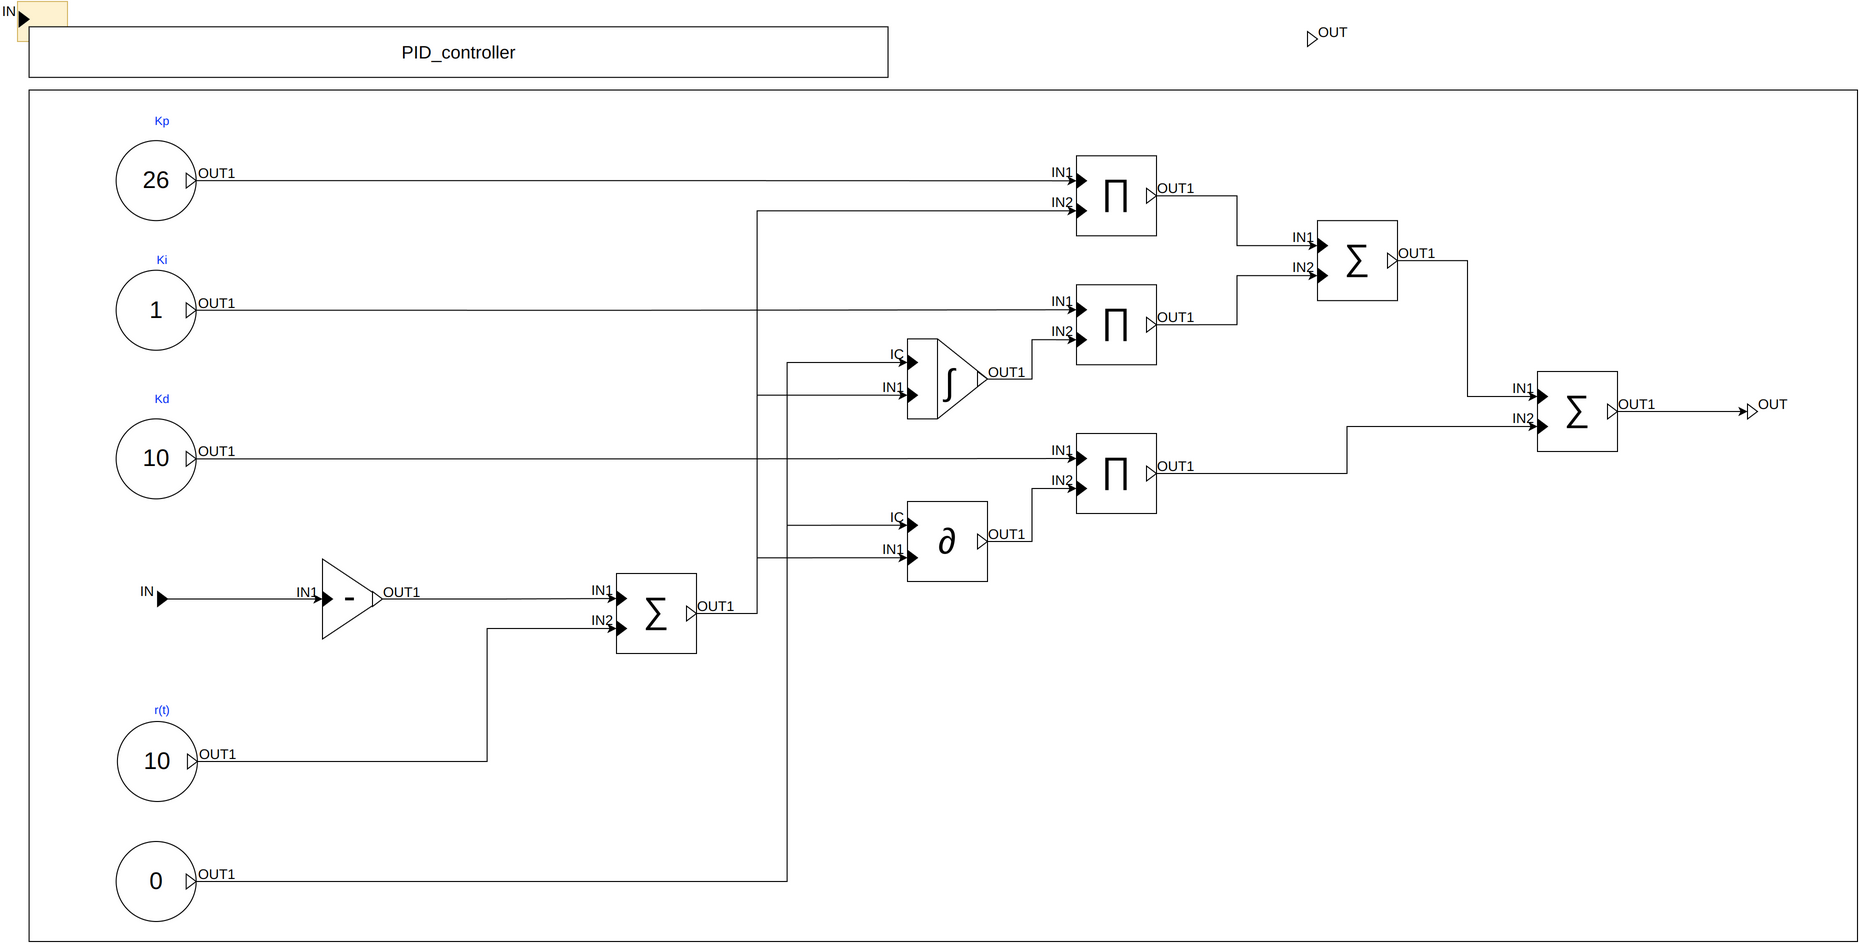
\includegraphics[width=0.75\linewidth]{Images/PID_controller.drawio.png}
    \caption{PID controller}
    \label{fig:PID-controller}
\end{figure}

\subsection{Co-simulate}
To combine the Plan FMU and controller FMU, we used the given orchestration script and modified it to connect the gantry system (Plan FMU) from assignment 1 to the new created CBD PID controller. When we ran the orchestration script we received a similar curve for our distance (x) as the one from assignment 1. But to our surprise they where not the same. After some debugging, we found out that when we set the derivation (Kd) value to 0 in both simulations (assignment 1 and 2), our curves where exactly the same. We found the problem after a couple of hours of debugging. We used the wrong derivation block in assignment 1 where the t=0 value of the derivation block was way larger than the value of the derivation of our CBD PID controller. This was because we used the Modelica.Blocks.Continuous.Derivative instead of the Modelica.Blocks.Continuous.Der, which is more precise. After changing this we got almost exactly the same values for our angle and distance between assignment 1 and our new orchestration script. This can be seen in figure \ref{fig:assigment1_plot} and \ref{fig:assigment2_plot}. This is the expected result, because we replaced the PID controller made in Modelica by an identical PID controller made using CBD's.

\begin{figure}
    \centering
    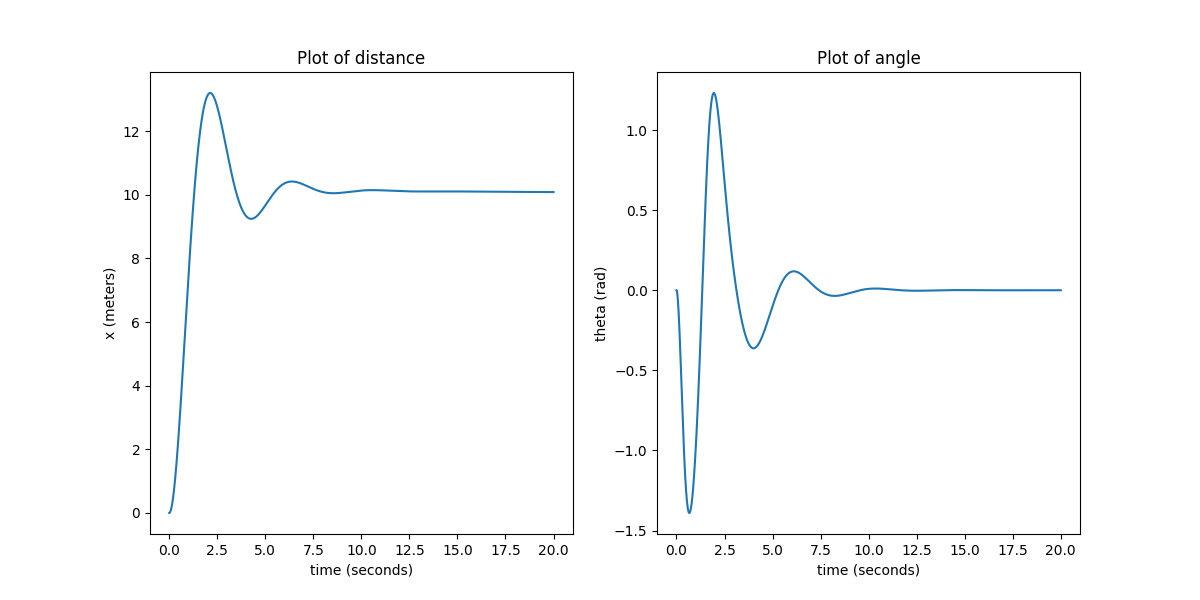
\includegraphics[width=0.75\linewidth]{Images/assigment1_plot.png}
    \caption{Plot distance and angle Modelica pid and Modelica FMU}
    \label{fig:assigment1_plot}
\end{figure}


\section{Jupyter notebook}
Because of the large amount of tools and steps in this lab, we created the assignment using a Jupyter notebook. All the steps to generate the CBD blocks, generate images, and generate the FMU's are present in this notebook.

\begin{figure}
    \centering
    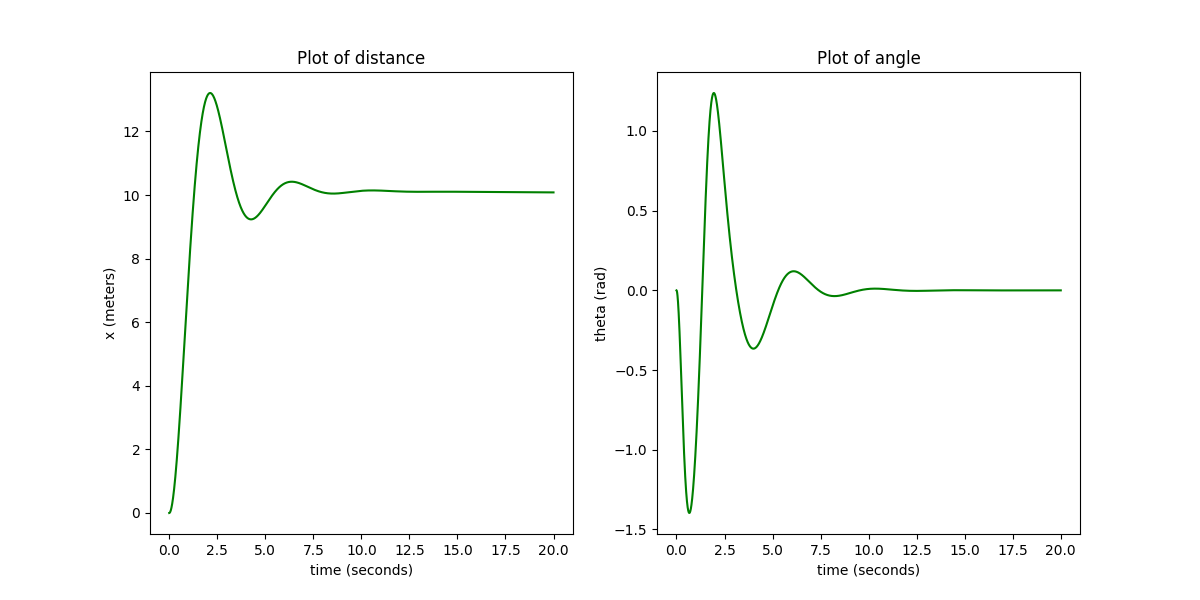
\includegraphics[width=0.75\linewidth]{Images/assigment2_plot.png}
    \caption{Plot distance and angle PID FMU and Plant FMU}
    \label{fig:assigment2_plot}
\end{figure}

\end{document}
